\documentclass{beamer}
\usepackage[utf8]{inputenc}
\usepackage{graphicx, epsfig}
\usepackage{amsmath,mathrsfs,amsfonts,amssymb}
\usepackage{floatflt}
\usepackage{epic,ecltree}
\usepackage{mathtext}
\usepackage{fancybox}
\usepackage{fancyhdr}
\usepackage{multirow}
\usepackage{enumerate}
\usepackage{epstopdf}
\usepackage{multicol}
\usepackage{algorithm}
\usepackage[noend]{algorithmic}
\usepackage{tikz}
\usepackage{blindtext}
\usepackage{multido}
\usetheme{default}%{Singapore}%{Warsaw}%{Warsaw}%{Darmstadt}
\usecolortheme{default}

\setbeamerfont{title}{size=\Huge}
\setbeamertemplate{footline}[frame number]{}

\setbeamertemplate{section in toc}[sections numbered]

\makeatletter
\newcommand\HUGE{\@setfontsize\Huge{35}{40}}
\makeatother    

\setbeamerfont{title}{size=\HUGE}
\beamertemplatenavigationsymbolsempty

\usetikzlibrary{arrows,shapes,positioning,shadows,trees}

\newcommand\myfootnote[1]{%
  \vspace{-0.5cm}%
  \tikz[remember picture,overlay]
  \draw (current page.south west) +(1in + \oddsidemargin,0.5em)
  node[anchor=south west,inner sep=0pt]{\parbox{\textwidth}{%
      \rlap{\rule{10em}{0.4pt}}\raggedright\scriptsize \textit{#1}}};}

\newcommand\myfootnotewithlink[2]{%
  \vspace{-0.5cm}%
  \tikz[remember picture,overlay]
  \draw (current page.south west) +(1in + \oddsidemargin,0.5em)
  node[anchor=south west,inner sep=0pt]{\parbox{\textwidth}{%
      \rlap{\rule{10em}{0.4pt}}\raggedright\scriptsize\href{#1}{\textit{#2}}}};}

\AtBeginSection[]
      {
      	\begin{frame}{Outline}
      		\tableofcontents[currentsection]
      	\end{frame}
      }
      \AtBeginSubsection[]{
      	\begin{frame}{Outline}
      		\tableofcontents[currentsection,currentsubsection]
      	\end{frame}
}

\newcounter{noscounter} % Используется для nextonslide команды (обнуляется только на новом слайде)
\newcounter{pcounter} % Используется для pause команды (обнуляется после использования eqpause)
\newcounter{diffcounter} % Считает количество pause после формулы

\newcommand{\nextonslide}[1]{%
  \stepcounter{noscounter}% Прибавляем счетчик nextonslide
  \stepcounter{pcounter}% Прибавляем счетчик pause
  \stepcounter{diffcounter}% Прибавляем счетчик diffcounter
  \onslide<\value{noscounter}->{#1}% Отображаем аргумент в скобках на слайде с номером noscounter
}
\newcommand{\resetonslide}{%
    \setcounter{noscounter}{1}% Сбрасываем счетчик nextonslide
    \setcounter{pcounter}{1}% Сбрасываем счетчик pause
    \setcounter{diffcounter}{0}% Сбрасываем счетчик diffcounter
}

\newcommand{\eqpause}{%
  \multido{\i=1+1}{\value{pcounter}}{\pause}% Повторяем pcounter раз команду pause
  \stepcounter{noscounter}% Прибавляем счетчик nextonslide
  \setcounter{pcounter}{1}% Сбрасываем счетчик pause
}

\newcommand{\eqpausediff}{% Вспомогательная команда, запускается автоматически после формул
  \multido{\i=1+1}{\value{diffcounter}}{\pause}% Повторяем diffcounter раз команду pause
  \addtocounter{pcounter}{-\value{diffcounter}}% Вычитаем из pcounter количество сделанных pause
  \setcounter{diffcounter}{0}% Сбрасываем счетчик diffcounter
}

\newcommand\AtEndBoth[2]{% Применяем команду к multline и multline*
  \AtEndEnvironment{#1}{#2}%
  \AtEndEnvironment{#1*}{#2}%
}

\AtEndBoth{align}{\eqpausediff}
\AtEndBoth{equation}{\eqpausediff}
\AtEndBoth{multline}{\eqpausediff}

\addtobeamertemplate{frametitle}{\resetonslide}{}% На каждом слайде сбрасываем счетчики

% latin bold lower
\newcommand{\ba}{\mathbf{a}} 
\newcommand{\bc}{\mathbf{c}} 
\newcommand{\be}{\mathbf{e}} 
\newcommand{\bff}{\mathbf{f}} % \bf - for bold type
\newcommand{\bg}{\mathbf{g}} 
\newcommand{\bh}{\mathbf{h}} 
\newcommand{\bp}{\mathbf{p}} 
\newcommand{\bq}{\mathbf{q}} 
\newcommand{\bt}{\mathbf{t}} 
\newcommand{\bs}{\mathbf{s}} 
\newcommand{\bu}{\mathbf{u}} 
\newcommand{\bv}{\mathbf{v}} 
\newcommand{\bw}{\mathbf{w}} 
\newcommand{\bx}{\mathbf{x}} 
\newcommand{\by}{\mathbf{y}} 
\newcommand{\bz}{\mathbf{z}} 

% latin bold upper
\newcommand{\bA}{\mathbf{A}} 
\newcommand{\bB}{\mathbf{B}} 
\newcommand{\bC}{\mathbf{C}} 
\newcommand{\bG}{\mathbf{G}} 
\newcommand{\bI}{\mathbf{I}} 
\newcommand{\bJ}{\mathbf{J}} 
\newcommand{\bL}{\mathbf{L}} 
\newcommand{\bM}{\mathbf{M}} 
\newcommand{\bP}{\mathbf{P}}
\newcommand{\bQ}{\mathbf{Q}} 
\newcommand{\bR}{\mathbf{R}} 
\newcommand{\bT}{\mathbf{T}} 
\newcommand{\bU}{\mathbf{U}} 
\newcommand{\bV}{\mathbf{V}} 
\newcommand{\bW}{\mathbf{W}} 
\newcommand{\bX}{\mathbf{X}} 
\newcommand{\bY}{\mathbf{Y}} 
\newcommand{\bZ}{\mathbf{Z}} 

% latin cal upper
\newcommand{\cF}{\mathcal{F}} 
\newcommand{\cG}{\mathcal{G}} 
\newcommand{\cI}{\mathcal{I}} 
\newcommand{\cL}{\mathcal{L}} 
\newcommand{\cM}{\mathcal{M}} 
\newcommand{\cN}{\mathcal{N}} 
\newcommand{\cP}{\mathcal{P}} 
\newcommand{\cS}{\mathcal{S}} 
\newcommand{\cT}{\mathcal{T}} 
\newcommand{\cW}{\mathcal{W}} 
\newcommand{\cX}{\mathcal{X}} 
\newcommand{\cZ}{\mathcal{Z}} 

% latin bb upper
\newcommand{\bbE}{\mathbb{E}} 
\newcommand{\bbI}{\mathbb{I}} 
\newcommand{\bbP}{\mathbb{P}} 
\newcommand{\bbR}{\mathbb{R}} 

% greek bold lower
\newcommand{\bepsilon}{\boldsymbol{\epsilon}} 
\newcommand{\btheta}{\boldsymbol{\theta}} 
\newcommand{\blambda}{\boldsymbol{\lambda}} 
\newcommand{\bpi}{\boldsymbol{\pi}} 
\newcommand{\bmu}{\boldsymbol{\mu}} 
\newcommand{\bsigma}{\boldsymbol{\sigma}} 
\newcommand{\bphi}{\boldsymbol{\phi}} 

% greek bold upper
\newcommand{\bSigma}{\boldsymbol{\Sigma}} 

\DeclareMathOperator*{\argmin}{arg\,min}
\DeclareMathOperator*{\argmax}{arg\,max}
\newcommand{\createdgmtitle}[1]{\title[\hbox to 56mm{Deep Generative Models  \hfill\insertframenumber\,/\,\inserttotalframenumber}]
	{\vspace{1cm} \\ \textbf{Deep Generative Models} \\ {\Huge Lecture #1}}
	\author{Roman Isachenko}
	\institute{
		Moscow Institute of Physics and Technology \\
		Yandex School of Data Analysis
	}
	\date{2025, Autumn}
}
\createdgmtitle{11}

\usepackage{tikz}

\usetikzlibrary{arrows,shapes,positioning,shadows,trees}
%--------------------------------------------------------------------------------
\begin{document}
%--------------------------------------------------------------------------------
\begin{frame}[noframenumbering,plain]
%\thispagestyle{empty}
\titlepage
\end{frame}
%=======
\begin{frame}{Recap of previous lecture}
	\begin{block}{DDPM objective}
		\vspace{-0.5cm}
		\[
			\bbE_{\pi(\bx_0)} \bbE_{t \sim U\{1, T\}}\bbE_{q(\bx_t | \bx_0)} \left[ {\color{olive}\frac{(1 - \alpha_t)^2}{2\tilde{\beta}_t \alpha_t}} \Bigl\|  \bs_{\btheta, t} (\bx_t) - \nabla_{\bx_t} \log q(\bx_t | \bx_0) \Bigr\|_2^2  \right]
		\]
		In practice, {\color{olive}this coefficient} is typically omitted.
	\end{block}
	\begin{block}{NCSN objective}
		\vspace{-0.3cm}
		\[
			\bbE_{\pi(\bx_0)} \bbE_{t \sim U\{1, T\}} \bbE_{q(\bx_t | \bx_0)}\bigl\| \bs_{\btheta, \sigma_t}(\bx_t) - \nabla_{\bx_t} \log q(\bx_t | \bx_0) \bigr\|^2_2 
		\]
		\vspace{-0.3cm}
	\end{block}
	\textbf{Note:} The objectives of DDPM and NCSN are almost identical; however, they differ in their sampling procedures:
	\begin{itemize}
		\item NCSN utilizes annealed Langevin dynamics;
		\item DDPM employs ancestral sampling.
	\end{itemize}
	\myfootnotewithlink{https://arxiv.org/abs/2006.11239}{Ho J. Denoising Diffusion Probabilistic Models, 2020}
	\end{frame}
%=======
\begin{frame}{Recap of previous lecture}
	\begin{block}{Unconditional generation}
		\vspace{-0.3cm}
		\[
			\bx_{t - 1} = \frac{1}{\sqrt{1 - \beta_t}} \cdot \bx_t + \frac{\beta_t}{\sqrt{1 - \beta_t}} \cdot {\color{teal} \nabla_{\bx_t} \log p(\bx_t | \btheta)} +  \sigma_t \cdot \bepsilon
		\]
		\vspace{-0.5cm}
	\end{block}
	\begin{block}{Conditional generation}
		\vspace{-0.5cm}
		\[
			\bx_{t - 1} =  \frac{1}{\sqrt{1 - \beta_t}}\cdot \bx_t +  \frac{\beta_t}{\sqrt{1 - \beta_t}}  \cdot  \nabla_{\bx_t} \log p(\bx_t | {\color{olive}\by}, \btheta) +  \sigma_t \cdot \bepsilon
		\]
		\vspace{-0.5cm}
	\end{block}
	\begin{block}{Conditional distribution}
		\vspace{-0.5cm}
		\begin{align*}
			{\color{olive}\nabla_{\bx_t} \log p(\bx_t | \by, \btheta)} &= \nabla_{\bx_t} \log p(\by | \bx_t) + {\color{violet}\nabla_{\bx_t} \log p(\bx_t | \btheta)}\\
			&= {\color{teal}\nabla_{\bx_t} \log p(\by | \bx_t)} {\color{violet}- \frac{\bepsilon_{\btheta, t}(\bx_t)}{\sqrt{1 - \bar{\alpha}_t}}}
		\end{align*}
		\vspace{-0.5cm}
	\end{block}
	Here, $p(\by | \bx_t)$ denotes the classifier operating on noisy samples (this must be trained separately).
	\myfootnotewithlink{https://arxiv.org/abs/2105.05233}{Dhariwal P., Nichol A. Diffusion Models Beat GANs on Image Synthesis, 2021}
\end{frame}
%=======
\begin{frame}{Recap of previous lecture}
	\begin{block}{Classifier-corrected noise prediction}
		\vspace{-0.3cm}
		\[
			\bepsilon_{\btheta, t}(\bx_t, \by) = \bepsilon_{\btheta, t}(\bx_t) - \sqrt{1 - \bar{\alpha}_t} \cdot \nabla_{\bx_t} \log p(\by | \bx_t)
		\]
		\vspace{-0.7cm}
	\end{block}
	\begin{block}{Guidance scale}
		\vspace{-0.3cm}
		\[
			{\color{olive}\bepsilon_{\btheta, t}(\bx_t, \by)} = \bepsilon_{\btheta, t}(\bx_t) - {\color{teal}\gamma} \cdot \sqrt{1 - \bar{\alpha}_t} \cdot \nabla_{\bx_t} \log p(\by | \bx_t)
		\]
		\vspace{-0.5cm}
	\end{block}
	\begin{itemize}
		\item Train DDPM as usual.
		\item Separately train an additional classifier $p(\by | \bx_t)$ on noisy samples $\bx_t$.
	\end{itemize}
	\begin{block}{Guided sampling}
		\vspace{-0.3cm}
		\[
			\bx_{t-1} = \frac{1}{\sqrt{\alpha_t}} \cdot \bx_t - \frac{1 - \alpha_t}{\sqrt{\alpha_t (1 - \bar{\alpha}_t)}} \cdot  {\color{olive}\bepsilon_{\btheta, t}(\bx_t, \by)} + \sigma_t \cdot \bepsilon
		\]
		\vspace{-0.3cm}
	\end{block}
	\textbf{Note:} The guidance scale $\gamma$ serves to sharpen the distribution $p(\by | \bx_t)$.
	\myfootnotewithlink{https://arxiv.org/abs/2105.05233}{Dhariwal P., Nichol A. Diffusion Models Beat GANs on Image Synthesis, 2021}
\end{frame}
%=======
\begin{frame}{Recap of previous lecture}
	The previous method requires training an additional classifier model $p(\by | \bx_t)$ on noisy data. Let us try to avoid this requirement.
	\[
		{\color{teal}\nabla_{\bx_t} \log p(\by | \bx_t)} =  \nabla_{\bx_t} \log p(\bx_t| \by, \btheta) -\nabla_{\bx_t} \log  p(\bx_t | \btheta)
	\]
	\vspace{-0.4cm}
	\begin{multline*}
		\nabla_{\bx_t}^{\gamma} \log p(\bx_t | \by, \btheta) = \nabla_{\bx_t} \log p(\bx_t | \btheta) + \gamma \cdot \nabla_{\bx_t} {\color{violet}\log p(\by | \bx_t)} = \\
		=  (1 - \gamma) \cdot  \nabla_{\bx_t} \log p(\bx_t | \btheta) + \gamma \cdot  \nabla_{\bx_t} \log p(\bx_t| \by, \btheta)
	\end{multline*}
	\vspace{-0.4cm}
	\begin{block}{Classifier-free-corrected noise prediction}
		\vspace{-0.3cm}
		\[
			\hat{\bepsilon}_{\btheta, t}(\bx_t, \by) = \gamma \cdot \bepsilon_{\btheta, t}(\bx_t, \by) + (1 - \gamma) \cdot \bepsilon_{\btheta, t}(\bx_t)
		\]
		\vspace{-0.5cm}
	\end{block}
	\begin{itemize}
		\item Train a single model $\bepsilon_{\btheta, t}(\bx_t, \by)$ on \textbf{supervised} data, alternating between real conditioning $\by$ and empty conditioning $\by = \emptyset$.
		\item Apply the model twice during inference.
	\end{itemize}
	\myfootnotewithlink{https://arxiv.org/abs/2207.12598}{Ho J., Salimans T. Classifier-Free Diffusion Guidance, 2022}
\end{frame}
%=======
\begin{frame}{Recap of previous lecture}
	\begin{block}{Continuous-in-time dynamics (Neural ODE)}
		\vspace{-0.5cm}
		\begin{align*}
			\frac{d \bx(t)}{dt} &= \bff_{\btheta}(\bx(t), t); \quad \text{with initial condition }\bx(t_0) = \bx_0. \\
			\bx(t_1) &= \int^{t_1}_{t_0} \bff_{\btheta}(\bx(t), t) d t  + \bx_0 \approx {\color{teal}\text{ODESolve}_f(\bx_0, \btheta, t_0, t_1)}.
		\end{align*}
		\vspace{-0.5cm}
	\end{block}
	Here, $\bff_{\btheta}: \bbR^m \times [t_0, t_1] \rightarrow \bbR^m$ is a vector field.
	\begin{block}{Euler update step (ODESolve)}
		\vspace{-0.3cm}
		\[
  			\bx(t + \Delta t) = \bx(t) + \Delta t \cdot \bff_{\btheta}(\bx(t), t)
		\]
	\end{block}
	\begin{itemize}
		\item The Euler method is the simplest version of ODESolve, but it is unstable in practice.
		\item More advanced numerical methods (e.g., Runge-Kutta methods) can be used instead of Euler.
	\end{itemize}
	\myfootnotewithlink{https://arxiv.org/abs/1806.07366}{Chen R. T. Q. et al. Neural Ordinary Differential Equations, 2018}   
\end{frame}
%=======
\begin{frame}{Recap of previous lecture}
	\vspace{-0.3cm}
	\[
 		\frac{d \bx(t)}{dt} = \bff_{\btheta}(\bx(t), t); \quad \text{with initial condition }\bx(t_0) = \bx_0
	\]
	\vspace{-0.3cm}
	\begin{itemize}
		\item Suppose $\bx(0)$ is a random variable with density~$p_0(\bx)$. Then $\bx(t)$ is a random variable with density~$p_t(\bx)$.
		\item $p_t(\bx) = p(\bx, t)$ describes the \textbf{probability path} between $p_0(\bx)$ and $p_1(\bx)$.
	\end{itemize}
	\vspace{-0.3cm}
	\begin{figure}
		\centering
		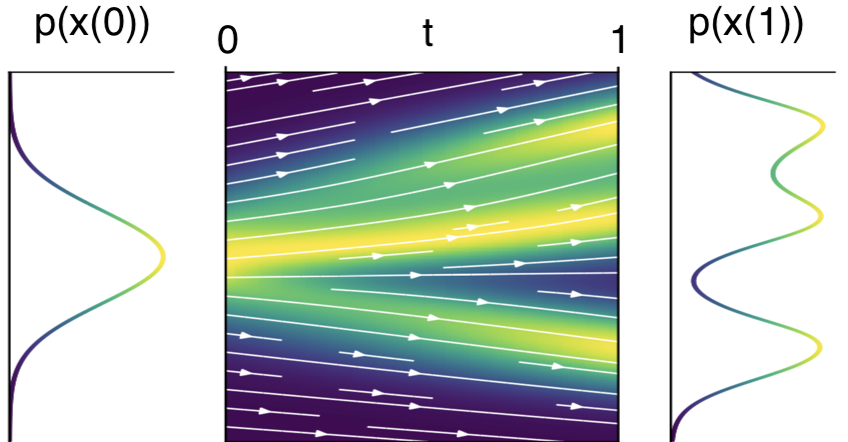
\includegraphics[width=0.7\linewidth]{figs/cnf_flow.png}
	\end{figure}
	\myfootnotewithlink{https://arxiv.org/abs/1810.01367}{Grathwohl W. et al. FFJORD: Free-form Continuous Dynamics for Scalable Reversible Generative Models, 2018}  
\end{frame}
%=======
\begin{frame}{Recap of previous lecture}
	\begin{block}{Theorem (Picard)}
		If $\bff$ is uniformly Lipschitz continuous in $\bx$ and continuous in $t$, then the ODE has a \textbf{unique} solution.
	\end{block}
	This means we can \textbf{uniquely invert} our ODE. 
	\begin{align*}
		\bx(1) &= \bx(0) + \int_{0}^{1} \bff_{\btheta}(\bx(t), t) dt \\
		\bx(0) &= \bx(1) + \int_{1}^{0} \bff_{\btheta}(\bx(t), t) dt
	\end{align*}
	\textbf{Note:} Unlike discrete-time NF, $\bff$ does not need to be invertible (uniqueness assures bijectivity).
	
	How can we compute $p_t(\bx)$ at any time $t$?
	\myfootnotewithlink{https://arxiv.org/abs/1806.07366}{Chen R. T. Q. et al. Neural Ordinary Differential Equations, 2018}   
\end{frame}
%=======
\begin{frame}{Outline}
	\tableofcontents
\end{frame}
%=======
\section{Continuity equation for NF log-likelihood}
%=======
\begin{frame}{Continuous-in-time NF}
	\begin{block}{Theorem (continuity equation)}
		If $\bff$ is uniformly Lipschitz continuous in $\bx$ and continuous in $t$, then
		\[
			\frac{d \log p_t(\bx(t))}{d t} = - \text{tr} \left( \frac{\partial \bff(\bx(t), t)}{\partial \bx(t)} \right)
		\]
		\vspace{-0.3cm}
	\end{block}
	This result states that, given $\bx_0 = \bx(0)$, the solution to the continuity equation provides the density $p_1(\bx(1))$.
	\begin{block}{Solution of continuity equation}
		\vspace{-0.3cm}
		\[
			\log p_1(\bx(1)) = \log p_0(\bx(0)) - {\color{teal}\int_{0}^{1} \text{tr}  \left( \frac{\partial \bff(\bx(t), t)}{\partial \bx(t)} \right) dt}.
		\]
	\end{block}
	\begin{itemize}
		\item This solution gives the density along the trajectory (not the total probability path).
		\item However, {\color{teal}the latter term} is difficult to estimate efficiently.
	 \end{itemize}
	\myfootnotewithlink{https://arxiv.org/abs/1806.07366}{Chen R. T. Q. et al. Neural Ordinary Differential Equations, 2018}   
\end{frame}
%=======
\section{SDE basics}
%=======
\begin{frame}{Stochastic differential equation (SDE)}
	Let us define a stochastic process $\bx(t)$ with initial condition $\bx(0) \sim p_0(\bx) = \pi(\bx)$:
	\[
		d\bx = \mathbf{f}(\bx, t) dt + g(t) d \bw
	\]
	\vspace{-0.5cm}
	\begin{itemize}
		 \item $\mathbf{f}(\bx, t): \bbR^m \times [0, 1] \rightarrow \bbR^m$ is the \textbf{drift} function of $\bx(t)$.
		 \item $g(t): \bbR \rightarrow \bbR$ is the \textbf{diffusion} function of $\bx(t)$.
		 \item $\bw(t)$ is the standard Wiener process (Brownian motion), characterized by:
		 \begin{enumerate}
		 	\item $\bw(0) = 0$ (almost surely);
		 	\item $\bw(t)$ has independent increments;
		 	\item $\bw(t)$ trajectories are continuous;
			 \item $\bw(t) - \bw(s) \sim \cN(0, (t - s) \bI)$ for $t > s$;
		 \end{enumerate}
		 \item $d \bw = \bw(t + dt) - \bw(t) = \cN(0, \bI \cdot dt ) = \bepsilon \cdot \sqrt{dt}$, with $\bepsilon \sim \cN(0, \bI)$.
		 \item If $g(t) = 0$, we recover the standard ODE.
	\end{itemize}
\end{frame}
%=======
\begin{frame}{Stochastic differential equation (SDE)}
	\[
		d\bx = \mathbf{f}(\bx, t) dt + g(t) d \bw
	\]
	\vspace{-0.3cm}
	\begin{itemize}
		\item Unlike ODEs, the initial condition $\bx(0)$ does not uniquely determine the trajectory of the process.
		\item There are two sources of randomness: the initial distribution $p_0(\bx)$ and the Wiener process $\bw(t)$.
	\end{itemize}
	\begin{block}{Discretization of SDE (Euler method) - SDESolve}
		\vspace{-0.3cm}
		\[
			\bx(t + dt) = \bx(t) + \bff(\bx(t), t) \cdot dt + g(t) \cdot \bepsilon \cdot \sqrt{dt}
		\]
		If $dt = 1$, then
		\vspace{-0.3cm}
		\[
			\bx_{t + 1} = \bx_t + \bff(\bx_t, t) + g(t) \cdot \bepsilon
		\]
		\vspace{-0.7cm}
	\end{block}
	\begin{itemize}
		\item At each time $t$, the process has density $p_t(\bx) = p(\bx, t)$.
		\item $p: \bbR^m \times [0, 1] \rightarrow \bbR_+$ defines a \textbf{probability path} from $p_0(\bx)$ to $p_1(\bx)$.
		\item How do we obtain the probability path $p_t(\bx)$ for $\bx(t)$?
	\end{itemize}
\end{frame}
%=======
\begin{frame}{Stochastic differential equation (SDE)}
	\vspace{-0.4cm}
	\[
		d\bx = \mathbf{f}(\bx, t) dt + g(t) d \bw, \quad d \bw = \bepsilon \cdot \sqrt{dt}, \quad \bepsilon \sim \cN(0, \bI).
	\]
	\vspace{-0.4cm}
 	\begin{block}{Theorem (Kolmogorov-Fokker-Planck)}
 		The evolution of the distribution $p_t(\bx)$ is governed by:
 		\vspace{-0.2cm}
 		\[
 			\frac{\partial p_t(\bx)}{\partial t} = - \text{div}\left(\bff(\bx, t) p_t(\bx)\right) + \frac{1}{2}g^2(t) \Delta_{\bx}p_t(\bx)
 		\]
 		Here
 		\[
 			\text{div} (\bv) = \sum_{i=1}^m \frac{\partial v_i(\bx)}{\partial x_i} = \text{tr}\left( \frac{\partial \bv(\bx)}{\partial \bx}  \right)
 		\]
 		\[
 			\Delta_{\bx}p_t(\bx) = \sum_{i=1}^m \frac{\partial^2 p_t(\bx)}{\partial x_i^2} = \text{tr}\left( \frac{\partial^2 p_t(\bx)}{\partial \bx^2}  \right)
 		\]
 		\[
 			\frac{\partial p_t(\bx)}{\partial t} = \text{tr}\left(- \frac{\partial}{\partial \bx} \bigl[ \mathbf{f}(\bx, t) p_t(\bx)\bigr] + \frac{1}{2} g^2(t) \frac{\partial^2 p_t(\bx)}{\partial \bx^2} \right)
 		\]
 	\end{block}
\end{frame}
%=======
\begin{frame}{Stochastic differential equation (SDE)}
 	\begin{block}{Theorem (Kolmogorov-Fokker-Planck)}
 		\vspace{-0.2cm}
 		\[
 			\frac{\partial p_t(\bx)}{\partial t} = \text{tr}\left(- \frac{\partial}{\partial \bx} \bigl[ \mathbf{f}(\bx, t) p_t(\bx)\bigr] + \frac{1}{2} g^2(t) \frac{\partial^2 p_t(\bx)}{\partial \bx^2} \right)
 		\]
 		\vspace{-0.2cm}
 	\end{block}
 	 \begin{itemize}
 	 	\item The KFP theorem uniquely determines the density $p_t(\bx)$.
 		 \item This generalizes the continuity equation previously used for continuous-time NF:
 	 	\[
 	 		\frac{d \log p_t(\bx(t))}{d t} = - \text{tr} \left( \frac{\partial \bff(\bx, t)}{\partial \bx} \right).
 	 	\]
 	 \end{itemize}
	\vspace{-0.3cm}
 	\begin{block}{Langevin SDE (special case)}
 		\vspace{-0.6cm}
 		\begin{align*}
 			d\bx &= {\color{violet}\mathbf{f}(\bx, t)} dt + {\color{teal}g(t)} d \bw \\
 			d \bx &= {\color{violet}\frac{1}{2} \frac{\partial}{\partial \bx} \log p_t(\bx)} d t + {\color{teal} 1 } \cdot d \bw
 		\end{align*}
 		\vspace{-0.4cm}
 	\end{block}
 	Let us apply the KFP theorem to this SDE.
\end{frame}
%=======
\begin{frame}{Langevin SDE (special case)}
	\[
		d \bx = \frac{1}{2} \frac{\partial}{\partial \bx} \log p_t(\bx) d t + 1 \cdot d \bw
	\]
	\begin{multline*}
		\frac{\partial p_t(\bx)}{\partial t} =  \text{tr} \left(- \frac{\partial}{\partial \bx}\left[ {\color{olive}p_t(\bx) \frac{1}{2} \frac{\partial}{\partial \bx} \log p_t(\bx)} \right]  + \frac{1}{2} \frac{\partial^2 p_t(\bx)}{\partial \bx^2} \right) = \\
		= \text{tr} \left(- \frac{\partial}{\partial \bx}\left[ {\color{olive}\frac{1}{2} \frac{\partial}{\partial \bx} p_t(\bx) } \right]  + \frac{1}{2} \frac{\partial^2 p_t(\bx)}{\partial \bx^2} \right) = 0
	\end{multline*}
	The density $p_t(\bx) = \text{const}(t)$! \\ If $\bx(0) \sim p_0(\bx)$, then $\bx(t) \sim p_0(\bx)$.
	\begin{block}{Discretized Langevin SDE}
		\vspace{-0.3cm}
		\[
			\bx_{t + 1} - \bx_t = \frac{\eta}{2} \cdot \frac{\partial}{\partial \bx} \log p_t(\bx) + \sqrt{\eta} \cdot \bepsilon, \quad \eta \approx dt.
		\]
		\vspace{-0.4cm}
	\end{block}
	\begin{block}{Langevin dynamic}
		\vspace{-0.3cm}
		\[
			\bx_{t + 1} = \bx_t + \frac{\eta}{2} \cdot \nabla_{\bx} \log p(\bx | \btheta) + \sqrt{\eta} \cdot \bepsilon, \quad \eta \approx dt.
		\]
		\vspace{-0.3cm}
	\end{block}
\end{frame}
%=======
\section{Probability flow ODE}
%=======
\begin{frame}{Probability flow ODE}
	\begin{block}{ODE and continuity equation}
		\vspace{-0.3cm}
		\[
			d\bx = \mathbf{f}(\bx, t) dt
		\]
		\[
			\frac{d \log p_t(\bx(t))}{d t} = - \text{tr} \left( \frac{\partial \bff_{\btheta}(\bx, t)}{\partial \bx} \right) 
			\quad  \Leftrightarrow  \quad 
 			\frac{\partial p_t(\bx)}{\partial t} = - \text{div}\left(\bff(\bx, t) p_t(\bx)\right)
 		\]
 		The only source of stochasticity is the distribution $p_0(\bx)$.
	\end{block}
	\begin{block}{SDE and KFP equation}
		\vspace{-0.3cm}
		\[
			d\bx = \mathbf{f}(\bx, t) dt + g(t) d \bw
		\]
 		\[
 			\frac{\partial p_t(\bx)}{\partial t} = - \text{div}\left(\bff(\bx, t) p_t(\bx)\right) + \frac{1}{2}g^2(t) \Delta_{\bx}p_t(\bx)
 		\]
 		We now have two sources of randomness: the initial distribution $p_0(\bx)$ and the Wiener process $\bw(t)$.
	\end{block}
	\myfootnotewithlink{https://arxiv.org/abs/2011.13456}{Song Y., et al. Score-Based Generative Modeling through Stochastic Differential Equations, 2020}
\end{frame}
%=======
\begin{frame}{Probability flow ODE}
	\begin{block}{Theorem}
		Assume the SDE $d\bx = \mathbf{f}(\bx, t) dt + g(t) d \bw$ induces the probability path~$p_t(\bx)$.
		Then there exists an ODE with the identical probability path $p_t(\bx)$, given by:
		\vspace{-0.3cm}
		\[
			d\bx = \left(\mathbf{f}(\bx, t) -\frac{1}{2} g^2(t) \frac{\partial}{\partial \bx} \log p_t(\bx) \right) dt
		\]
		\vspace{-0.7cm}
	\end{block}
	\begin{figure}
		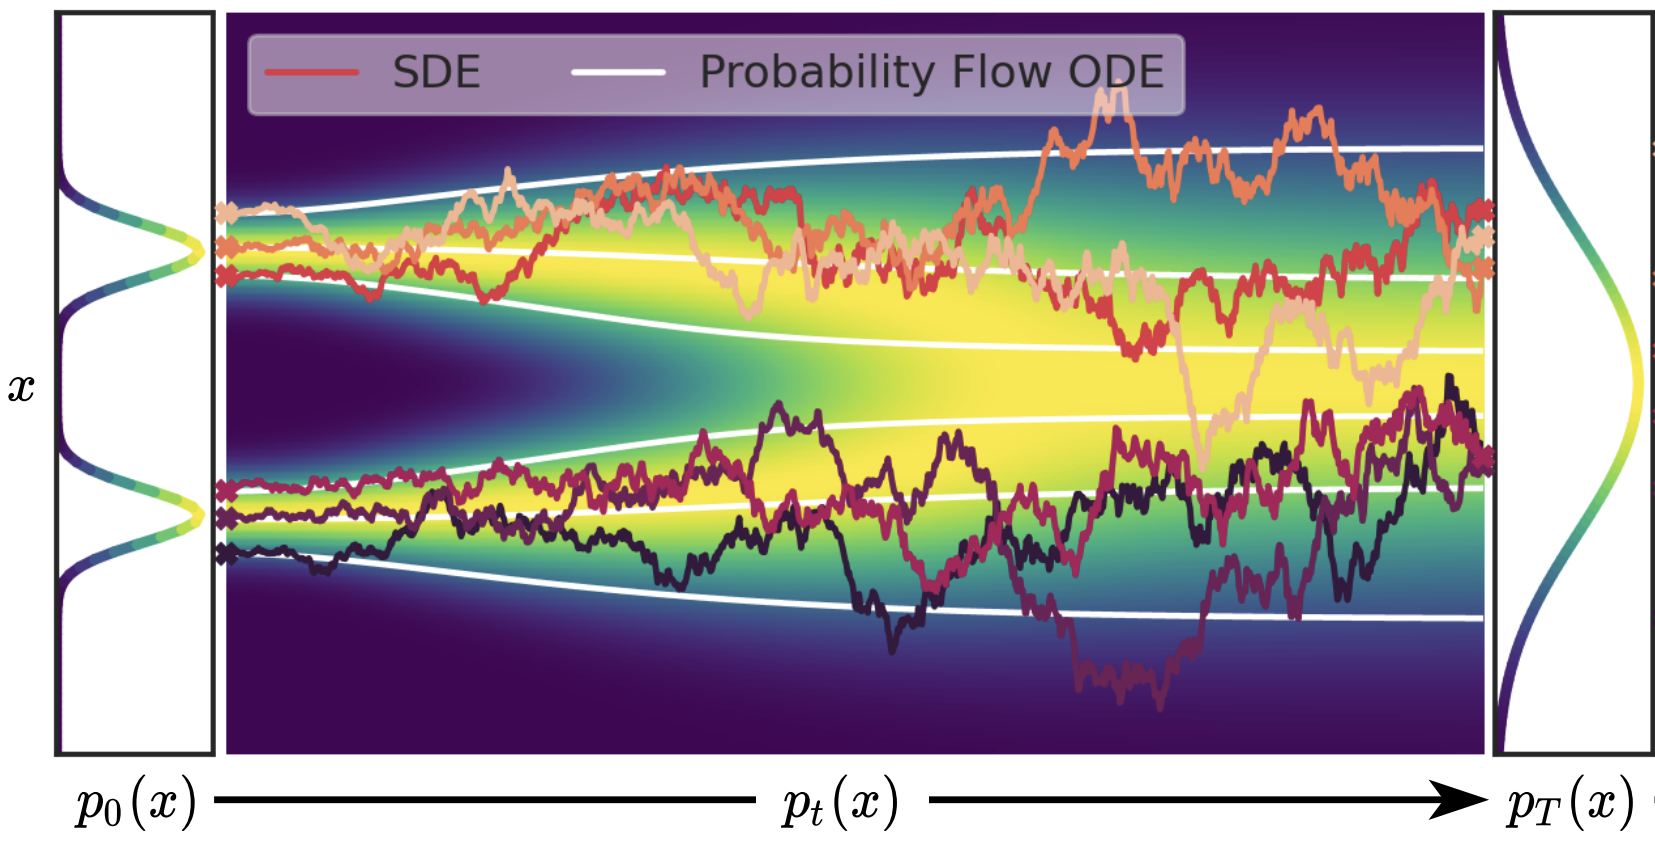
\includegraphics[width=0.75\linewidth]{figs/probability_flow}
	\end{figure}
	\myfootnotewithlink{https://arxiv.org/abs/2011.13456}{Song Y., et al. Score-Based Generative Modeling through Stochastic Differential Equations, 2020}
\end{frame}
%=======
\begin{frame}{Probability flow ODE}
	\begin{block}{Theorem}
		Assume the SDE $d\bx = \mathbf{f}(\bx, t) dt + g(t) d \bw$ induces the probability path~$p_t(\bx)$.
		Then there exists an ODE with the identical probability path $p_t(\bx)$, given by:
		\vspace{-0.3cm}
		\[
			d\bx = \left(\mathbf{f}(\bx, t) -\frac{1}{2} g^2(t) \frac{\partial}{\partial \bx} \log p_t(\bx) \right) dt
		\]
		\vspace{-0.7cm}
	\end{block}
	\begin{block}{Proof}
 		\vspace{-0.7cm}
 		{\small
 		\begin{multline*}
 			\frac{\partial p_t(\bx)}{\partial t} = \text{tr}\left(- \frac{\partial}{\partial \bx} \bigl[ \mathbf{f}(\bx, t) p_t(\bx)\bigr] + \frac{1}{2} g^2(t) \frac{\partial^2 p_t(\bx)}{\partial \bx^2} \right) = \\
 			=  \text{tr}\left(- \frac{\partial}{\partial \bx} \left[ \mathbf{f}(\bx, t) p_t(\bx) - \frac{1}{2} g^2(t) {\color{violet}\frac{\partial p_t(\bx)}{\partial \bx}} \right]  \right) = \\
			 =  \text{tr}\left(- \frac{\partial}{\partial \bx} \left[ \mathbf{f}(\bx, t) p_t(\bx) - \frac{1}{2} g^2(t) {\color{violet}p_t(\bx) \frac{\partial}{\partial \bx} \log p_t(\bx)} \right]  \right)= \\
		  =  \text{tr}\left(- \frac{\partial}{\partial \bx} \left[ \left( {\color{teal}\mathbf{f}(\bx, t) - \frac{1}{2} g^2(t) \frac{\partial}{\partial \bx} \log p_t(\bx)}\right) p_t(\bx) \right]  \right)
 		\end{multline*}
 		}
 	\end{block}
	\myfootnotewithlink{https://arxiv.org/abs/2011.13456}{Song Y., et al. Score-Based Generative Modeling through Stochastic Differential Equations, 2020}
\end{frame}
%=======
\begin{frame}{Probability flow ODE}
	\begin{block}{Proof (continued)}
 		\vspace{-0.7cm}
 		\begin{multline*}
 			\frac{\partial p_t(\bx)}{\partial t} =  \text{tr}\left(- \frac{\partial}{\partial \bx} \left[ \left( {\color{teal}\mathbf{f}(\bx, t) - \frac{1}{2} g^2(t) \frac{\partial}{\partial \bx}\log p_t(\bx)}\right) p_t(\bx) \right]  \right) =\\
 			  =  \text{tr}\left(- \frac{\partial}{\partial \bx} \left[ {\color{teal}\tilde{\mathbf{f}}(\bx, t)} p_t(\bx) \right]  \right) = -  \text{div}\left(\tilde{\mathbf{f}}(\bx, t) p_t(\bx)\right) 
 		\end{multline*}
		\[
			\tilde{\bff}(\bx, t) = \bff(\bx, t) -\frac{1}{2} g^2(t) \frac{\partial}{\partial \bx} \log p_t(\bx); \quad \tilde{g}(t) = 0
		\]
	 	\[
	 		d \bx = \tilde{\bff}(\bx, t) dt + 0 \cdot d \bw = \left(\bff(\bx, t) -\frac{1}{2} g^2(t) \frac{\partial}{\partial \bx} \log p_t(\bx) \right) dt
	 	\]
		\[
			\frac{\partial p_t(\bx)}{\partial t} = - \text{div}\left(\tilde{\mathbf{f}}(\bx, t) p_t(\bx)\right) + \frac{1}{2}\tilde{g}^2(t) \Delta_{\bx}p_t(\bx)
		\]
 	\end{block}
	\myfootnotewithlink{https://arxiv.org/abs/2011.13456}{Song Y., et al. Score-Based Generative Modeling through Stochastic Differential Equations, 2020}
\end{frame}
%=======
\begin{frame}{Probability flow ODE}
	\vspace{-0.5cm}
	\begin{align*}
		d\bx &= \mathbf{f}(\bx, t) dt + g(t) d \bw - \text{SDE} \\
		d\bx &= \left(\mathbf{f}(\bx, t) -\frac{1}{2} g^2(t) \frac{\partial}{\partial \bx} \log p_t(\bx) \right) dt  - \text{probability flow ODE}
	\end{align*}
	\vspace{-0.3cm}
	\begin{itemize}
		\item The term $\bs(\bx, t) = \frac{\partial}{\partial \bx} \log p_t(\bx)$ is the score function in continuous time.
		\item The ODE has more stable trajectories.
	\end{itemize}
	\begin{figure}
		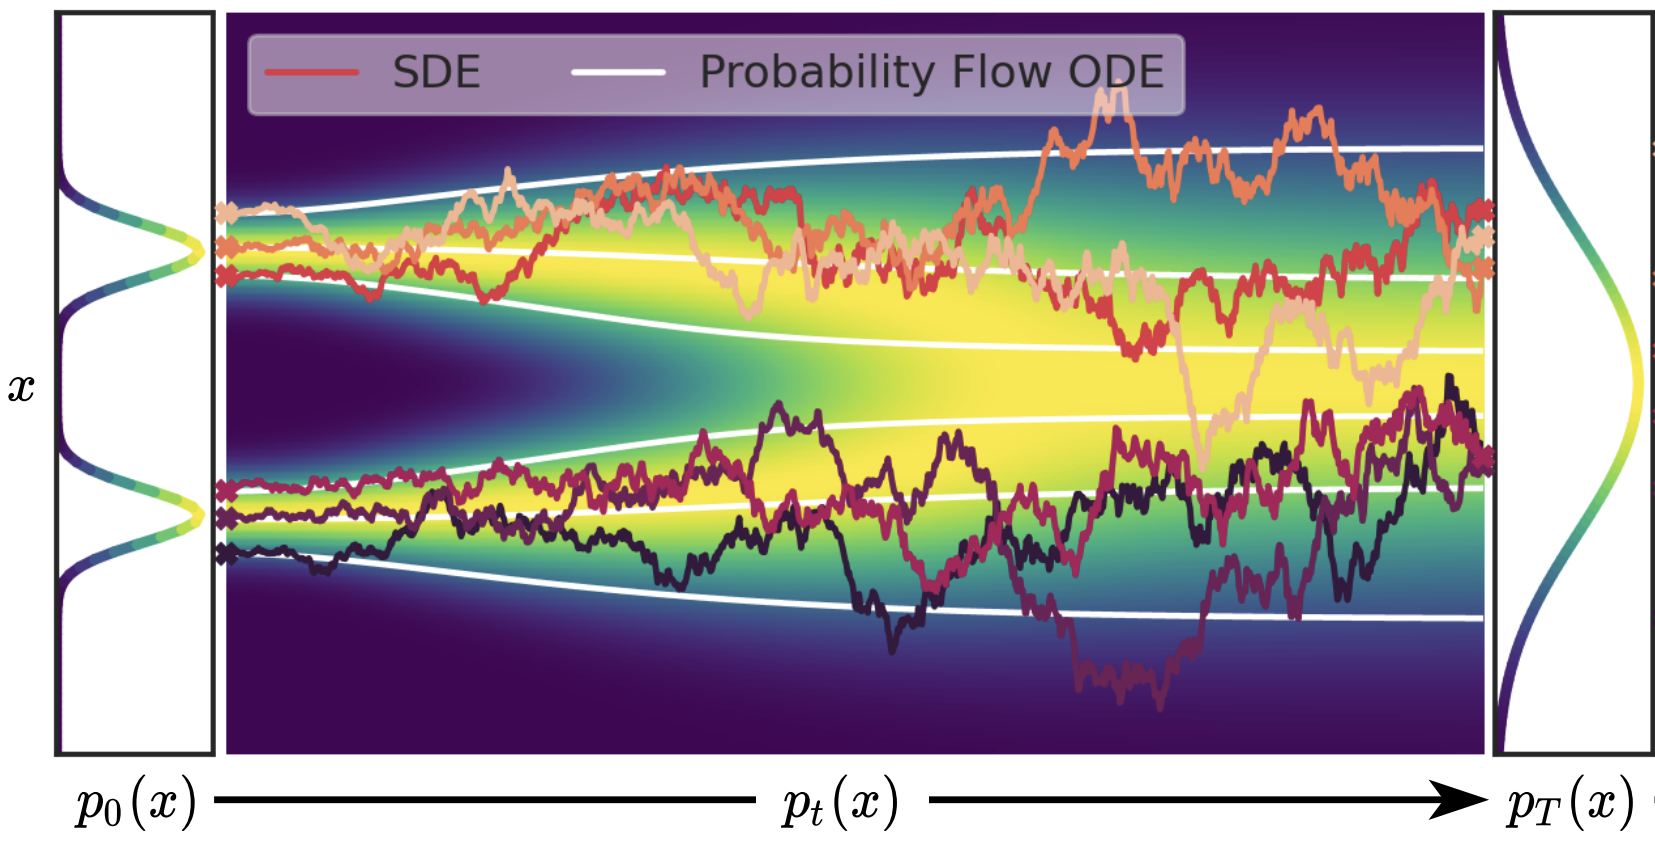
\includegraphics[width=0.75\linewidth]{figs/probability_flow}
	\end{figure}
	\myfootnotewithlink{https://arxiv.org/abs/2011.13456}{Song Y., et al. Score-Based Generative Modeling through Stochastic Differential Equations, 2020}
\end{frame}
%=======
\section{Reverse SDE}
%=======
\begin{frame}{Reverse SDE}
	\vspace{-0.3cm}
	\[
		d\bx = \mathbf{f}(\bx, t) dt, \quad \bx(t + dt) = \bx(t) + \mathbf{f}(\bx, t) dt
	\]
	Here $dt$ may be $>0$ or $<0$. 
	\begin{block}{Reverse ODE}
		Let $\tau = 1 - t$ ($d\tau = -dt$).
		\vspace{-0.3cm}
		\[
			d\bx = - \bff(\bx, 1 - \tau) d \tau
		\]
	\end{block}
	\vspace{-0.5cm}
	\begin{itemize}
		\item How do we reverse the SDE $d\bx = \mathbf{f}(\bx, t) dt + g(t) d \bw$? 
		\item The Wiener process introduces randomness that must be reversed.
	\end{itemize}
	\vspace{-0.3cm}
	\begin{block}{Theorem}
		There exists a reverse SDE for $d\bx = \mathbf{f}(\bx, t) dt + g(t) d \bw$, given by:
		\vspace{-0.3cm}
		\[
			d\bx = \left(\mathbf{f}(\bx, t) {\color{violet}- g^2(t) \frac{\partial}{\partial \bx}\log p_t(\bx)}\right) dt + g(t) d \bw
		\]
		\vspace{-0.5cm} \\
		where $dt < 0$.
	\end{block}
	\myfootnotewithlink{https://arxiv.org/abs/2011.13456}{Song Y., et al. Score-Based Generative Modeling through Stochastic Differential Equations, 2020}
\end{frame}
%=======
\begin{frame}{Reverse SDE}
	\begin{block}{Theorem}
		There exists a reverse SDE for $d\bx = \mathbf{f}(\bx, t) dt + g(t) d \bw$, given by:
		\vspace{-0.3cm}
		\[
			d\bx = \left(\mathbf{f}(\bx, t) {\color{violet}- g^2(t) \frac{\partial}{\partial \bx}\log p_t(\bx)}\right) dt + g(t) d \bw
		\]
		\vspace{-0.5cm} \\
		where $dt < 0$.
	\end{block}
	\textbf{Note:} Here we also observe the score function $\bs(\bx, t) = \frac{\partial}{\partial \bx} \log p_t(\bx)$.
	\begin{block}{Sketch of the proof}
		\begin{itemize}
			\item Convert the initial SDE to a probability flow ODE.
			\item Reverse the probability flow ODE.
			\item Convert the reversed probability flow ODE to a reverse SDE.
		\end{itemize}
	\end{block}
	\myfootnotewithlink{https://arxiv.org/abs/2011.13456}{Song Y., et al. Score-Based Generative Modeling through Stochastic Differential Equations, 2020}
\end{frame}
%=======
\begin{frame}{Reverse SDE}
	\begin{block}{Proof}
		\begin{itemize}
			\item Convert the initial SDE to a probability flow ODE:
			\vspace{-0.1cm}
			{\footnotesize
			\begin{align*}
				d\bx &= \mathbf{f}(\bx, t) dt + g(t) d \bw \\
				d\bx &= \left(\mathbf{f}(\bx, t) -\frac{1}{2} g^2(t) \frac{\partial}{\partial \bx} \log p_t(\bx) \right) dt
			\end{align*}
			}
			\item Reverse the probability flow ODE:
			\vspace{-0.1cm}
			{\footnotesize
			\begin{align*}
				d\bx &= \left(\mathbf{f}(\bx, t) -\frac{1}{2} g^2(t) \frac{\partial}{\partial \bx} \log p_t(\bx) \right) dt \\
				d\bx &= \left(- \mathbf{f}(\bx, 1 - \tau) + \frac{1}{2} g^2(1 - \tau) \frac{\partial}{\partial \bx} \log p_{1 - \tau}(\bx) \right) d \tau
			\end{align*}
			}
			\item Convert the reversed probability flow ODE to a reverse SDE:
			\vspace{-0.1cm}
			{\footnotesize
			\begin{align*}
				d\bx &= \left(- \mathbf{f}(\bx, 1 - \tau) + \frac{1}{2} g^2(1 - \tau) \frac{\partial}{\partial \bx} \log p_{1 - \tau}(\bx) \right) d \tau \\
				d\bx &= \left(- \mathbf{f}(\bx, 1 - \tau) + g^2(1 - \tau) \frac{\partial}{\partial \bx} \log p_{1 - \tau}(\bx) \right) d\tau + g(1 - \tau) d \bw
			\end{align*}
			}
		\end{itemize}
	\end{block}
	\myfootnotewithlink{https://arxiv.org/abs/2011.13456}{Song Y., et al. Score-Based Generative Modeling through Stochastic Differential Equations, 2020}
\end{frame}
%=======
\begin{frame}{Reverse SDE}
	\begin{block}{Theorem}
		There exists a reverse SDE for $d\bx = \mathbf{f}(\bx, t) dt + g(t) d \bw$, given by:
		\vspace{-0.3cm}
		\[
			d\bx = \left(\mathbf{f}(\bx, t) {\color{violet}- g^2(t) \frac{\partial}{\partial \bx}\log p_t(\bx)}\right) dt + g(t) d \bw
		\]
		\vspace{-0.5cm} \\
		where $dt < 0$.
	\end{block}
	\begin{block}{Proof (continued)}
		\vspace{-0.7cm}
		\[
			d\bx = \left(- \mathbf{f}(\bx, 1 - \tau) + g^2(1 - \tau) \frac{\partial}{\partial \bx} \log p_{1 - \tau}(\bx) \right) d \tau + g(1 - \tau) d \bw
		\]
		\[
			d\bx = \left(\mathbf{f}(\bx, t) - g^2(t) \frac{\partial}{\partial \bx}\log p_t(\bx)\right) dt + g(t) d \bw
		\]
		Here $d\tau > 0$ and $dt < 0$.
	\end{block}
	\myfootnotewithlink{https://arxiv.org/abs/2011.13456}{Song Y., et al. Score-Based Generative Modeling through Stochastic Differential Equations, 2020}
\end{frame}
%=======
\begin{frame}{Reverse SDE}
	\vspace{-0.5cm}
	\begin{align*}
		d\bx &= \mathbf{f}(\bx, t) dt + g(t) d \bw - \text{SDE} \\
		d\bx &= \left(\mathbf{f}(\bx, t) -\frac{1}{2} g^2(t) \frac{\partial}{\partial \bx} \log p_t(\bx) \right) dt - \text{probability flow ODE} \\
		d\bx &= \left(\mathbf{f}(\bx, t) - g^2(t) \frac{\partial}{\partial \bx}\log p_t(\bx)\right) dt + g(t) d \bw - \text{reverse SDE}
	\end{align*}
	\vspace{-0.5cm}
	\begin{itemize}
		\item This framework allows us to transform one distribution into another via an SDE with a specified probability path $p_t(\bx)$.
		\item We can invert this process using the score function.
	\end{itemize}
	\vspace{-0.3cm}
	\begin{figure}
		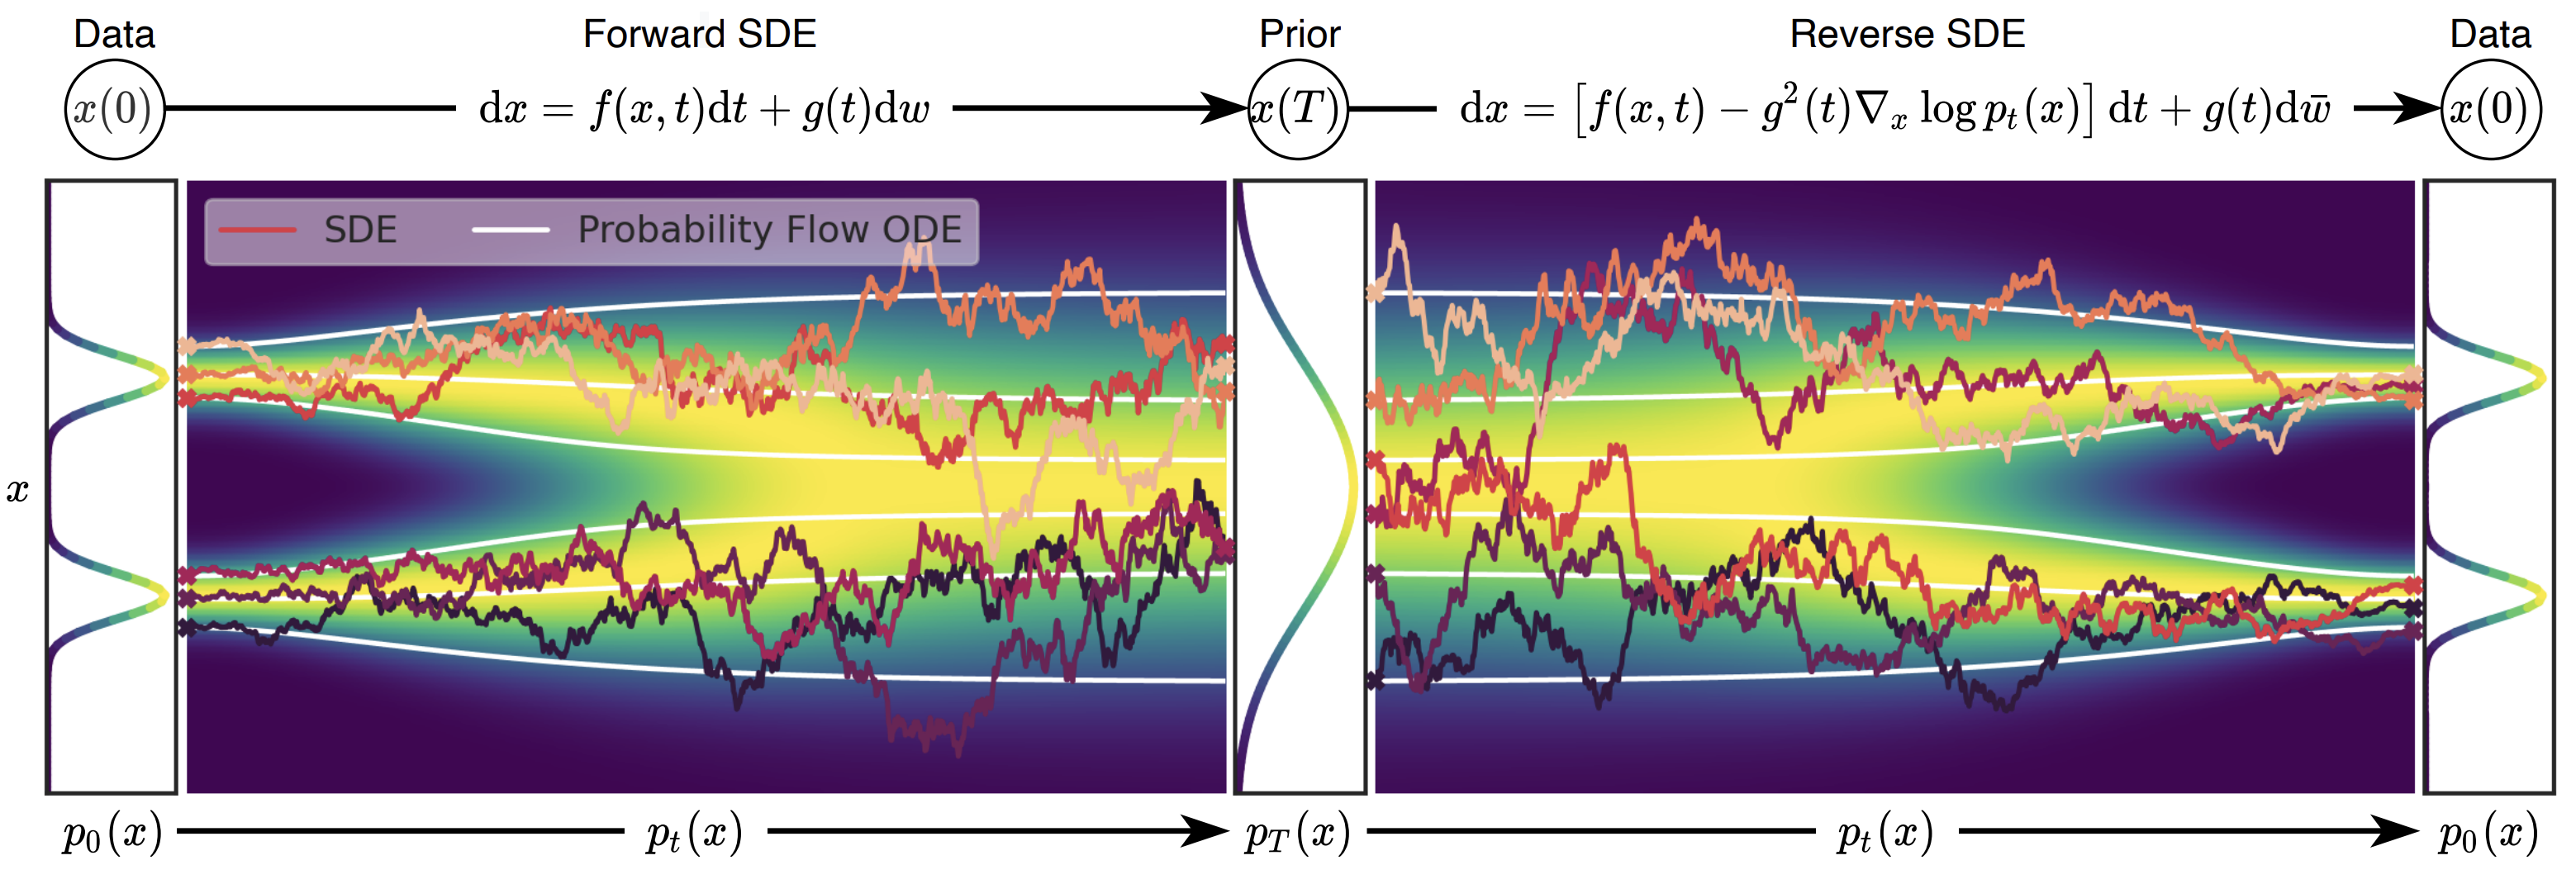
\includegraphics[width=0.9\linewidth]{figs/sde}
	\end{figure}
	\myfootnotewithlink{https://arxiv.org/abs/2011.13456}{Song Y., et al. Score-Based Generative Modeling through Stochastic Differential Equations, 2020}
\end{frame}
%=======
\begin{frame}{Summary}
	\begin{itemize}
		\item The continuity equation allows the computation of $\log p(\bx, t)$ at any time $t$.
		\vfill
		\item An SDE defines a stochastic process with drift and diffusion terms; ODEs are a special case of SDEs.
		\vfill
		\item The KFP equation describes the dynamics of the probability function for the SDE. 
		\vfill
		\item The Langevin SDE preserves a constant probability path.
		\vfill
		\item For every SDE, there exists a special probability flow ODE that follows the same probability path.
		\vfill
		\item SDEs can be reversed using the score function.
	\end{itemize}
\end{frame}
\end{document}